\chapter{Corrosão e proteção}\label{ch:b2:corrosion}

Deixe uma gota de água salgada sobre um pedaço limpo de aço. Depois de um dia,
o metal está corroído com pites no centro da gota, enquanto a ferrugem se
formou em um anel perto da borda, onde o oxigênio do ar se dissolve. O ferro
se dissolve onde há menos oxigênio, e o oxigênio é reduzido onde há mais: a
gota é uma pilha que ninguém construiu, em curto-circuito através do próprio
metal. Este capítulo lê a corrosão nas \omterm{def:b2:current-potential-curves:ie-curve}{curvas corrente--potencial}, explica por
que uma chapa galvanizada riscada não enferruja enquanto uma lata estanhada
riscada enferruja, e projeta a proteção de um duto enterrado.

\begin{recall}
O volume do 1.º ano: diagramas E--pH dos metais e seus domínios de imunidade,
corrosão e \omterm{def:b2:corrosion:passivation}{passivação} (``se uma camada protege é uma questão cinética'').
\Cref{ch:b2:current-potential-curves}: \omterm{def:b2:current-potential-curves:ie-curve}{curvas corrente--potencial}, \omterm{def:b2:current-potential-curves:limiting-current}{correntes
limite}. \Cref{ch:b2:batteries-electrolysis}: o \omterm{def:b2:batteries-electrolysis:mixed-potential}{potencial misto}. O volume
escolar: a corrosão, a ferrugem, a galvanização.
\end{recall}

\begin{omfigure}
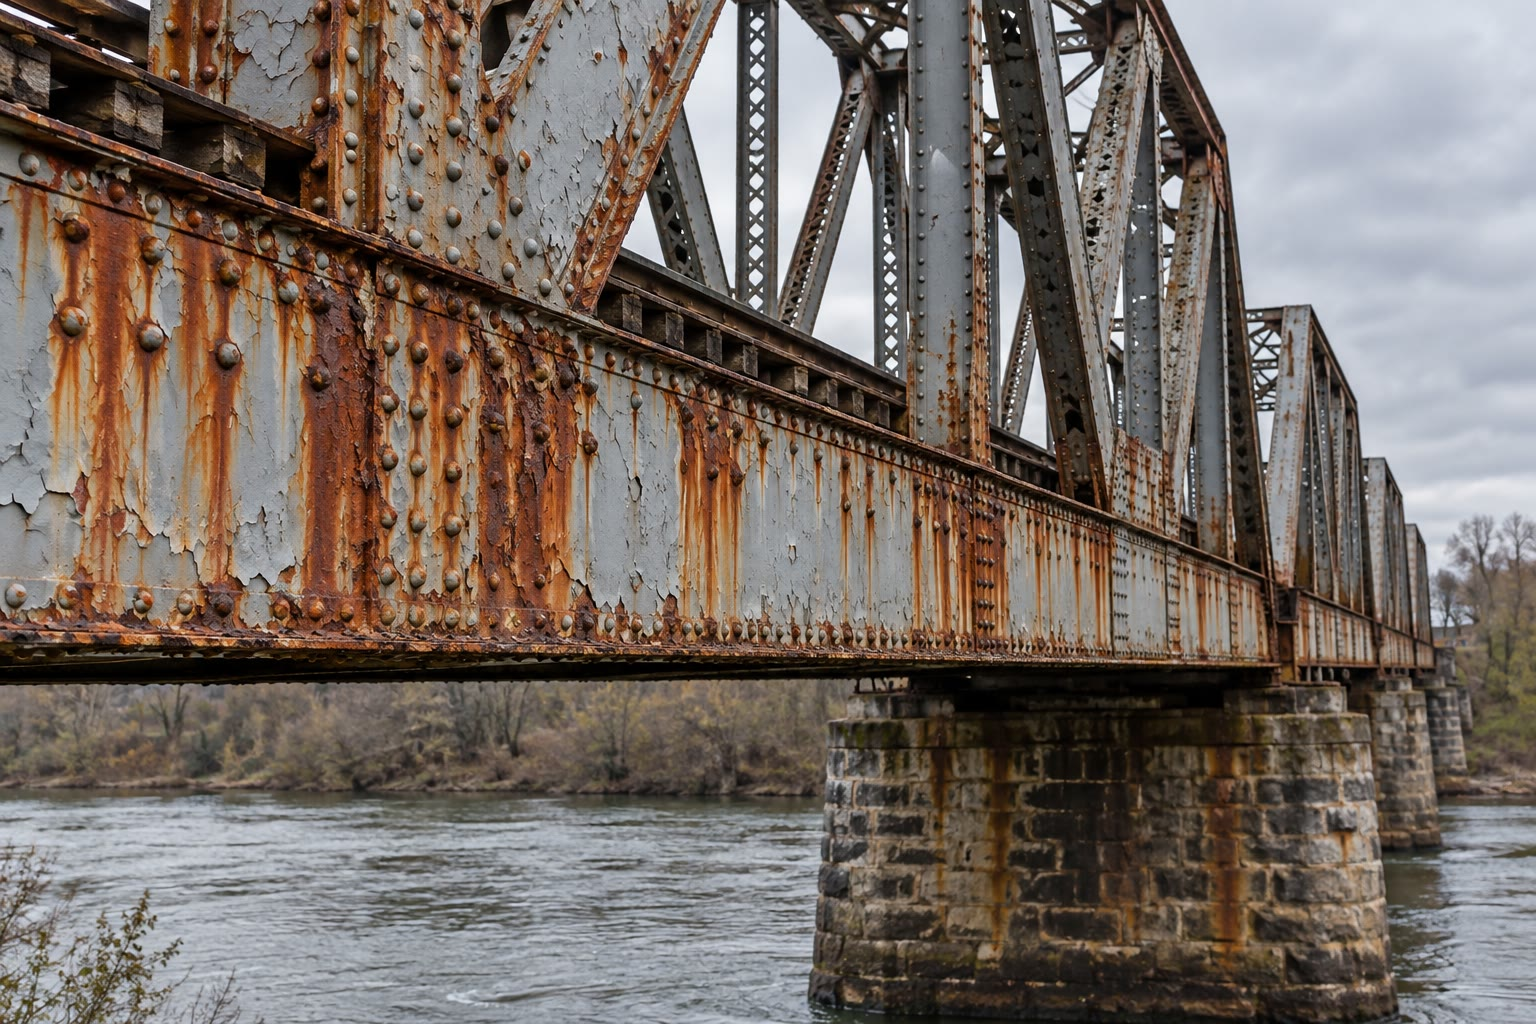
\includegraphics[width=0.62\linewidth]{images/book3/ai/b2-12-rusty-bridge.jpg}

{\small Uma velha ponte ferroviária rebitada. Escorrimentos de ferrugem descem
dos rebites e das juntas, onde a água e o oxigênio permanecem por mais tempo e
a pintura falha primeiro.}
\end{omfigure}

\section{A corrosão úmida como pilha em curto-circuito}

Na água que contém oxigênio dissolvido, o ferro é oxidado, \ce{Fe -> Fe^2+ + 2e-},
e os elétrons são captados no mesmo pedaço de metal pela redução do
dioxigênio, \ce{O2 + 2H2O + 4e- -> 4OH-} (em meio ácido, também por \ce{2H+ + 2e- -> H2}). Os
íons ferro(II) e os íons hidróxido se encontram na água, e a oxidação
posterior pelo ar transforma seu precipitado em ferrugem, um óxido de
ferro(III) hidratado.

\begin{definition}[Corrosão uniforme]\label{def:b2:corrosion:uniform}
A \emph{corrosão uniforme}\index{corrosao uniforme@corrosão uniforme} é a corrosão de um metal
cuja oxidação e a redução do oxidante ocorrem em sítios distribuídos de modo
homogêneo por sua superfície. O \emph{potencial de corrosão}\index{potencial de corrosao@potencial de corrosão}
é o \omterm{def:b2:batteries-electrolysis:mixed-potential}{potencial misto} que o metal assume então, e a
\emph{corrente de corrosão}\index{corrente de corrosao@corrente de corrosão}, a \omterm{def:b2:current-potential-curves:ie-curve}{corrente anódica}
da oxidação do metal nesse potencial.
\end{definition}

\begin{omfigure}
\begin{tikzpicture}
\begin{axis}[omie, width=0.82\linewidth, height=5.6cm, xmin=-1.1, xmax=0.5,
  ymin=-1.6, ymax=1.6, xlabel={$E$}, ylabel={$i$}, clip=true, clip mode=individual,
  axis y line=left]
\addplot[omanodic] table[x=E, y=i] {figdata/out/bachelor-2-ie-curves-i-Fe.dat};
\addplot[omcathodic] table[x=E, y=i] {figdata/out/bachelor-2-ie-curves-i-O2.dat};
\addplot[omcathodic, densely dashed] table[x=E, y=i, y expr=-\thisrow{i}] {figdata/out/bachelor-2-ie-curves-i-O2.dat};
\draw[densely dotted] (axis cs:-0.394,-1.0) -- (axis cs:-0.394,1.0);
\fill (axis cs:-0.394,1.0) circle (1.4pt);
\node[font=\scriptsize, anchor=south east] at (axis cs:-0.40,1.02) {$i_{\text{corr}}$};
\node[font=\scriptsize, anchor=north west] at (axis cs:-0.39,-0.03) {$E_{\text{corr}}$};
\node[font=\scriptsize, omThm, anchor=west] at (axis cs:-0.35,1.4) {\ce{Fe} $\to$ \ce{Fe^2+}};
\node[font=\scriptsize, omDef, anchor=north west] at (axis cs:-0.75,-1.05) {\ce{O2} $\to$ \ce{OH-}, patamar de difusão};
\end{axis}
\end{tikzpicture}

{\small O diagrama de Evans do ferro em água neutra aerada (curvas modelo). A
curva catódica do dioxigênio também é desenhada refletida para cima
(tracejada): o \omterm{def:b2:corrosion:uniform}{potencial de corrosão} é onde ela encontra a curva anódica do
ferro. Como a redução do dioxigênio atingiu ali seu patamar de difusão, a
\omterm{def:b2:corrosion:uniform}{corrente de corrosão} é igual à \omterm{def:b2:current-potential-curves:limiting-current}{corrente limite} do oxigênio: agitar ou arejar
a água faz o ferro corroer mais depressa.}
\end{omfigure}

\begin{proposition}[Velocidade de corrosão]\label{prop:b2:corrosion:rate}
Um metal de massa molar $M$ e massa específica $\rho$, oxidado com $n$
elétrons por átomo sob uma densidade de \omterm{def:b2:corrosion:uniform}{corrente de corrosão} $j_{\text{corr}}$
(corrente por unidade de área), perde por unidade de área e de tempo a massa
$j_{\text{corr}}M/(nF)$, isto é, uma espessura
\[
  \frac{de}{dt} = \frac{j_{\text{corr}}\,M}{nF\rho} .
\]
\end{proposition}

\begin{proof}
Pela \cref{prop:b2:current-potential-curves:current-rate}, a densidade de
\omterm{def:b2:current-potential-curves:ie-curve}{corrente anódica} $j_{\text{corr}}$ oxida $j_{\text{corr}}/(nF)$ mols de metal por unidade de
área e de tempo; multiplique por $M$ para a massa e divida por $\rho$ para a espessura.
\end{proof}

\begin{example}[Ferro a \qty{10}{\micro A/cm^2}]\label{ex:b2:corrosion:rate}
Com $j = \qty{0.10}{A/m^2}$, $M = \qty{55.845}{g/mol}$, $n = 2$, $\rho =
\qty{7.87}{g/cm^3}$: $de/dt = 0.10 \times 55.845/(2 \times 96\,485 \times 7.87
\times 10^6) = \qty{3.7e-12}{m/s}$, isto é, \qty{0.12}{mm} por ano.
% ledger: aw:Fe, rho:Fe, const:F
\end{example}

\section{Corrosão diferencial}

\begin{definition}[Corrosão diferencial]\label{def:b2:corrosion:differential}
A \emph{corrosão diferencial}\index{corrosao diferencial@corrosão diferencial} é uma corrosão na
qual os sítios anódicos e catódicos estão separados, sendo o metal oxidado
preferencialmente nos sítios anódicos. É \emph{corrosão
galvânica}\index{corrosao galvanica@corrosão galvânica} quando dois metais diferentes em contato
elétrico compartilham o mesmo eletrólito, e \emph{aeração
diferencial}\index{aeracao diferencial@aeração diferencial} quando um mesmo metal está exposto a águas de
diferentes teores de oxigênio.
\end{definition}

\begin{proposition}[Dois metais em contato]\label{prop:b2:corrosion:galvanic}
Quando dois metais em contato elétrico mergulham na mesma água aerada, eles
assumem um único \omterm{def:b2:batteries-electrolysis:mixed-potential}{potencial misto}. O metal cujo \omterm{def:b2:corrosion:uniform}{potencial de corrosão} é mais
baixo torna-se o ânodo e corrói mais depressa do que sozinho; o outro
torna-se um cátodo, sobre o qual o dioxigênio é reduzido, e fica protegido.
\end{proposition}

\begin{proof}
Ligados por um condutor de resistência desprezível, os dois metais estão ao
mesmo potencial, onde a soma de todas as \omterm{def:b2:current-potential-curves:ie-curve}{correntes anódicas} é igual a menos a
soma de todas as \omterm{def:b2:current-potential-curves:ie-curve}{correntes catódicas}. A curva anódica do metal menos nobre
sobe primeiro; no potencial comum, ela transporta quase toda a \omterm{def:b2:current-potential-curves:ie-curve}{corrente
anódica}, e o oxigênio é reduzido em toda a superfície molhada, inclusive no
metal mais nobre, cuja própria \omterm{def:b2:current-potential-curves:ie-curve}{corrente anódica} é desprezível ali.
\end{proof}

\begin{omfigure}
\begin{tikzpicture}
\begin{axis}[omie, width=0.82\linewidth, height=5.6cm, xmin=-1.1, xmax=0.5,
  ymin=-2.4, ymax=2.4, xlabel={$E$}, ylabel={$i$}, clip=true, clip mode=individual,
  axis y line=left]
\addplot[omanodic] table[x=E, y=i] {figdata/out/bachelor-2-ie-curves-i-Fe.dat};
\addplot[omanodic, densely dashed] table[x=E, y=i] {figdata/out/bachelor-2-ie-curves-j-Zn.dat};
\addplot[omcathodic] table[x=E, y=i] {figdata/out/bachelor-2-ie-curves-i-O2.dat};
\addplot[omcathodic, densely dashed] table[x=E, y=i] {figdata/out/bachelor-2-ie-curves-j-O2Cu.dat};
\fill (axis cs:-0.394,1.0) circle (1.4pt);
\fill (axis cs:-0.794,1.0) circle (1.4pt);
\fill (axis cs:-0.366,2.0) circle (1.4pt);
\draw[densely dotted] (axis cs:-1.1,1.0) -- (axis cs:-0.394,1.0);
\draw[densely dotted] (axis cs:-1.1,2.0) -- (axis cs:-0.366,2.0);
\node[font=\scriptsize, anchor=south west] at (axis cs:-0.38,0.95) {ferro sozinho};
\node[font=\scriptsize, anchor=west] at (axis cs:-0.35,2.0) {ferro + cobre};
\node[font=\scriptsize, anchor=south east] at (axis cs:-0.80,1.05) {ferro + zinco};
\node[font=\scriptsize, omThm, anchor=north west] at (axis cs:-0.98,0.75) {zinco};
\node[font=\scriptsize, omThm, anchor=north west] at (axis cs:-0.55,0.75) {ferro};
\node[font=\scriptsize, omDef, anchor=north east] at (axis cs:0.45,-2.05) {\ce{O2} sobre ferro + cobre};
\node[font=\scriptsize, omDef, anchor=north east] at (axis cs:0.45,-1.05) {\ce{O2} sobre ferro};
\end{axis}
\end{tikzpicture}

{\small O ferro acoplado a outros metais (curvas modelo). Com o zinco, o
potencial comum cai até onde o zinco transporta a \omterm{def:b2:current-potential-curves:ie-curve}{corrente anódica}: o ferro
fica protegido, o zinco corrói. Com o cobre, a área catódica para o oxigênio
dobra: a \omterm{def:b2:corrosion:uniform}{corrente de corrosão} do ferro também dobra.}
\end{omfigure}

\begin{proposition}[Aeração diferencial]\label{prop:b2:corrosion:aeration}
Em um metal exposto a águas de diferentes teores de oxigênio, a zona menos
aerada é anódica e corrói; a zona mais aerada é catódica.
\end{proposition}

\begin{proof}
Onde o teor de oxigênio é mais alto, o par \ce{O2}/\ce{OH-} tem um potencial
de Nernst mais alto e uma \omterm{def:b2:current-potential-curves:limiting-current}{corrente limite} maior: a curva catódica fica mais
alta e vai mais longe. O metal, um único condutor, se estabiliza em um só
potencial; a grande \omterm{def:b2:current-potential-curves:ie-curve}{corrente catódica} disponível na zona aerada precisa ser
equilibrada por uma \omterm{def:b2:current-potential-curves:ie-curve}{corrente anódica}, que circula onde o metal pode ser
oxidado com pouca concorrência da redução do oxigênio: a zona pouco aerada.
A oxidação se concentra ali.
\end{proof}

\begin{omfigure}
\begin{tikzpicture}[font=\small, >={Stealth}]
  \fill[black!20] (-4.2,-0.7) rectangle (4.2,0);
  \node[font=\scriptsize] at (3.7,-0.35) {aço};
  \fill[omDef!15] (-3.4,0) .. controls (-2.9,2.2) and (2.9,2.2) .. (3.4,0) -- cycle;
  \draw[thick, omDef] (-3.4,0) .. controls (-2.9,2.2) and (2.9,2.2) .. (3.4,0);
  \fill[omProp!80] (-0.7,0) arc[start angle=180, end angle=360, x radius=0.7, y radius=0.22] -- cycle;
  \fill[brown!70!black] (-1.9,0.12) ellipse (0.45 and 0.11);
  \fill[brown!70!black] (1.9,0.12) ellipse (0.45 and 0.11);
  \node[font=\scriptsize, align=center] at (0,2.45) {\ce{O2} do ar};
  \draw[->, thick, omDef] (-1.0,2.25) -- (-2.6,0.35);
  \draw[->, thick, omDef] (1.0,2.25) -- (2.6,0.35);
  \node[font=\scriptsize, align=center, anchor=east] at (-4.1,1.3) {cátodo\\ (borda)};
  \draw[->, thin] (-4.1,1.3) -- (-3.05,0.12);
  \node[font=\scriptsize, align=center, anchor=west] at (4.1,1.3) {anel de ferrugem};
  \draw[->, thin] (4.1,1.3) -- (2.3,0.2);
  \draw[->, omThm] (-0.4,-0.3) .. controls (-1.2,-0.5) and (-2.4,-0.5) .. (-3.0,-0.15);
  \draw[->, omThm] (0.4,-0.3) .. controls (1.2,-0.5) and (2.4,-0.5) .. (3.0,-0.15);
  \draw[->, thin] (0,-1.05) -- (0,-0.25);
  \node[font=\scriptsize, anchor=north] at (0,-1.05) {ânodo (centro): \ce{Fe -> Fe^2+ + 2e-}};
  \node[font=\scriptsize, omThm, anchor=north] at (0,-1.45) {os elétrons circulam pelo aço até a borda};
  \node[font=\scriptsize, anchor=north] at (0,-1.85) {cátodo (borda): \ce{O2 + 2H2O + 4e- -> 4OH-}};
\end{tikzpicture}

{\small A gota de Evans sobre o aço, esquemática. O oxigênio se dissolve na
superfície e chega ao metal sobretudo perto da borda fina da gota, que se
torna o cátodo; o centro, privado de oxigênio, é o ânodo e sofre pites. Os
íons ferro(II) e os íons hidróxido se encontram entre os dois, onde a ferrugem
precipita em anel.}
\end{omfigure}

O mesmo mecanismo ataca as frestas, as partes de uma estrutura sob um depósito
ou uma junta de vedação, e uma estaca de aço no mar logo abaixo da linha
d'água, onde a água é menos aerada que na superfície.

\begin{method}[Diagnosticar uma corrosão]\label{met:b2:corrosion:diagnose}
\begin{enumerate}
  \item Liste os metais em contato e o eletrólito; verifique se estão
        ligados eletricamente.
  \item Para dois metais, o de \omterm{def:b2:corrosion:uniform}{potencial de corrosão} mais baixo (em geral o
        de potencial padrão mais baixo) é o ânodo.
  \item Para um único metal, encontre as zonas menos aeradas (frestas, sob
        depósitos, o fundo de uma gota): elas são anódicas.
  \item A velocidade é fixada pela reação catódica (suprimento de oxigênio,
        área do cátodo): um ânodo pequeno sobre um cátodo grande corrói depressa.
\end{enumerate}
\end{method}

\section{Passivação}

\begin{definition}[Passivação]\label{def:b2:corrosion:passivation}
A \emph{passivação}\index{passivacao@passivação} é a forte diminuição da velocidade de
corrosão de um metal quando ele é recoberto por uma camada fina, compacta e
aderente de seu óxido, o \emph{filme passivo}\index{filme passivo}, que o separa da
solução. Diz-se que um metal nesse estado está passivo.
\end{definition}

\begin{proposition}[O patamar passivo]\label{prop:b2:corrosion:passivity}
A curva anódica de um metal passivável sobe a partir de seu \omterm{def:b2:corrosion:uniform}{potencial de
corrosão}, atinge um pico e depois cai para uma corrente passiva pequena e
quase constante em uma faixa de potenciais, antes de subir de novo em
potenciais altos (região transpassiva: oxidação do filme ou da água). O estado
passivo pode se romper localmente, por exemplo sob íons cloreto, formando pites.
\end{proposition}

\begin{proof}[Raciocínio]
Em \omterm{def:b2:current-potential-curves:overpotential}{sobretensões} baixas, o metal nu se dissolve cada vez mais depressa. Além de
um limiar, o óxido se torna estável na superfície (o domínio de \omterm{def:b2:corrosion:passivation}{passivação} do
diagrama E--pH) e forma um filme através do qual os íons se movem apenas
lentamente: a corrente desaba até esse pequeno fluxo. Em potenciais altos, o
próprio filme é oxidado a espécies solúveis, ou a água é oxidada sobre ele. Os
íons cloreto, pequenos e fortemente complexantes, podem dissolver o filme em
pontos fracos, onde o metal nu passa a corroer como um pequeno ânodo diante
de um enorme cátodo passivo. A forma da curva é aqui um modelo.
\end{proof}

\begin{omfigure}
\begin{tikzpicture}
\begin{axis}[omie, width=0.82\linewidth, height=5.4cm, xmin=-0.7, xmax=1.5,
  ymin=-0.1, ymax=1.3, xlabel={$E$}, ylabel={$i$}, clip=true, clip mode=individual,
  axis y line=left]
\addplot[omanodic] table[x=E, y=i] {figdata/out/bachelor-2-ie-curves-k.dat};
\node[font=\scriptsize, anchor=south] at (axis cs:-0.33,1.0) {ativo};
\node[font=\scriptsize, anchor=south] at (axis cs:0.5,0.06) {patamar passivo};
\node[font=\scriptsize, anchor=east] at (axis cs:1.25,0.9) {transpassivo};
\draw[<-, thin] (axis cs:-0.2,0.55) -- (axis cs:0.15,0.7) node[right, font=\scriptsize] {o filme se forma};
\end{axis}
\end{tikzpicture}

{\small Curva anódica de um metal passivável (modelo). A corrente, grande
enquanto o metal nu se dissolve, desaba quando o \omterm{def:b2:corrosion:passivation}{filme passivo} se forma e
permanece pequena em uma ampla faixa de potenciais antes da subida
transpassiva.}
\end{omfigure}

Os aços inoxidáveis contêm cromo suficiente para formar um \omterm{def:b2:corrosion:passivation}{filme passivo} de
óxido de cromo que se regenera ao ar; o alumínio é protegido por seu filme de
alumina, o que torna um metal muito abaixo do hidrogênio na série utilizável
em esquadrias de janela e latas de bebida. O cobre fica verde ao ar livre,
sendo a pátina uma camada de sais básicos de cobre que retarda o ataque.

\begin{omfigure}
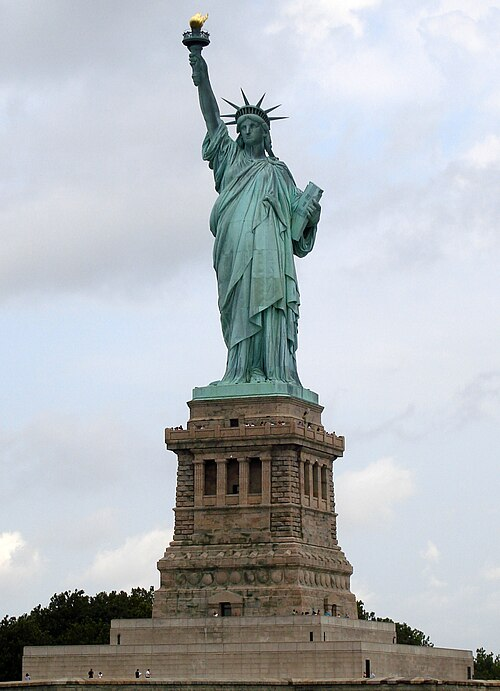
\includegraphics[width=0.32\linewidth]{images/book3/liberty.jpg}

{\small Uma estátua de cobre com mais de um século: sua pele de fina chapa de
cobre ficou verde, recoberta por uma pátina de sais básicos de cobre que
protege o metal por baixo. (Fotografia: Elcobbola, domínio público, Wikimedia
Commons.)}
\end{omfigure}

\section{Proteção}

A corrosão é combatida separando o metal da água e do oxigênio (pintura,
plástico, esmalte ou uma camada de outro metal), mudando o meio (retirando o
oxigênio, adicionando inibidores que se adsorvem no metal) ou deslocando o
potencial do metal para seu domínio de imunidade.

\begin{definition}[Proteção catódica]\label{def:b2:corrosion:protection}
A \emph{proteção catódica}\index{protecao catodica@proteção catódica} abaixa o potencial de uma
estrutura metálica até que sua oxidação cesse, fazendo dela o cátodo de uma
pilha. A pilha pode ser formada com um \emph{ânodo de sacrifício}\index{anodo de sacrificio@ânodo de sacrifício},
um metal menos nobre (zinco, magnésio, ligas de alumínio) ligado à
estrutura e consumido em seu lugar, ou impulsionada por um gerador, na
\emph{proteção por corrente impressa}\index{protecao por corrente impressa@proteção por corrente impressa}, sendo o
ânodo então um eletrodo inerte enterrado nas proximidades.
\end{definition}

\begin{proposition}[Duração de um ânodo de sacrifício]\label{prop:b2:corrosion:anode-life}
Um \omterm{def:b2:corrosion:protection}{ânodo de sacrifício} de massa $m$ e massa molar $M$, oxidado com $n$ elétrons
e um rendimento $\eta$ (a fração do metal que produz corrente útil, o resto
corroendo por conta própria), fornece uma corrente $I$ durante um tempo
\[
  t = \frac{\eta\,m\,nF}{M I} .
\]
\end{proposition}

\begin{proof}
A carga útil é $\eta\,(m/M)\,nF$; divida pela corrente.
\end{proof}

\begin{omfigure}
\begin{tikzpicture}[font=\small, >={Stealth}]
  \fill[brown!20] (-4.2,-2.4) rectangle (4.2,0);
  \draw[thick] (-4.2,0) -- (4.2,0);
  \node[font=\scriptsize, anchor=south west] at (-4.2,0) {solo};
  \fill[black!40] (-3.5,-1.6) rectangle (3.5,-1.2);
  \node[font=\scriptsize, white] at (0,-1.4) {tubo de aço (cátodo)};
  % sacrificial anode
  \fill[black!65] (-3.2,-2.3) rectangle (-2.2,-1.95);
  \node[font=\scriptsize, anchor=north] at (-2.7,-2.3) {ânodo de Mg};
  \draw[thick] (-2.7,-1.95) -- (-2.7,-1.6);
  \draw[->, omProp, thick] (-2.2,-2.12) -- (-1.4,-1.7);
  \node[font=\scriptsize, omProp, anchor=west] at (-1.9,-2.2) {corrente no solo};
  % impressed current
  \draw[thick, rounded corners] (1.8,0.4) rectangle (3.2,1.2);
  \node[font=\scriptsize] at (2.5,0.8) {\tiny retificador};
  \fill[black!65] (3.4,-2.3) rectangle (3.9,-1.8);
  \node[font=\scriptsize, anchor=north] at (3.65,-2.3) {ânodo inerte};
  \draw[thick] (3.2,0.8) -- (3.65,0.8) -- (3.65,-1.8);
  \draw[thick] (1.8,0.8) -- (1.2,0.8) -- (1.2,-1.2);
  \node[font=\scriptsize, anchor=south] at (3.65,0.85) {$+$};
  \node[font=\scriptsize, anchor=south] at (1.2,0.85) {$-$};
  \node[font=\scriptsize, align=center] at (-2.7,0.8) {ânodo de sacrifício};
  \node[font=\scriptsize, align=center] at (2.5,1.55) {corrente impressa};
\end{tikzpicture}

{\small \omterm{def:b2:corrosion:protection}{Proteção catódica} de um duto enterrado, esquemática. À esquerda: um
ânodo de magnésio, ligado por fio ao duto, corrói em seu lugar. À direita: um
retificador impulsiona uma corrente de um ânodo inerte, através do solo, até
o duto.}
\end{omfigure}

\begin{omfigure}
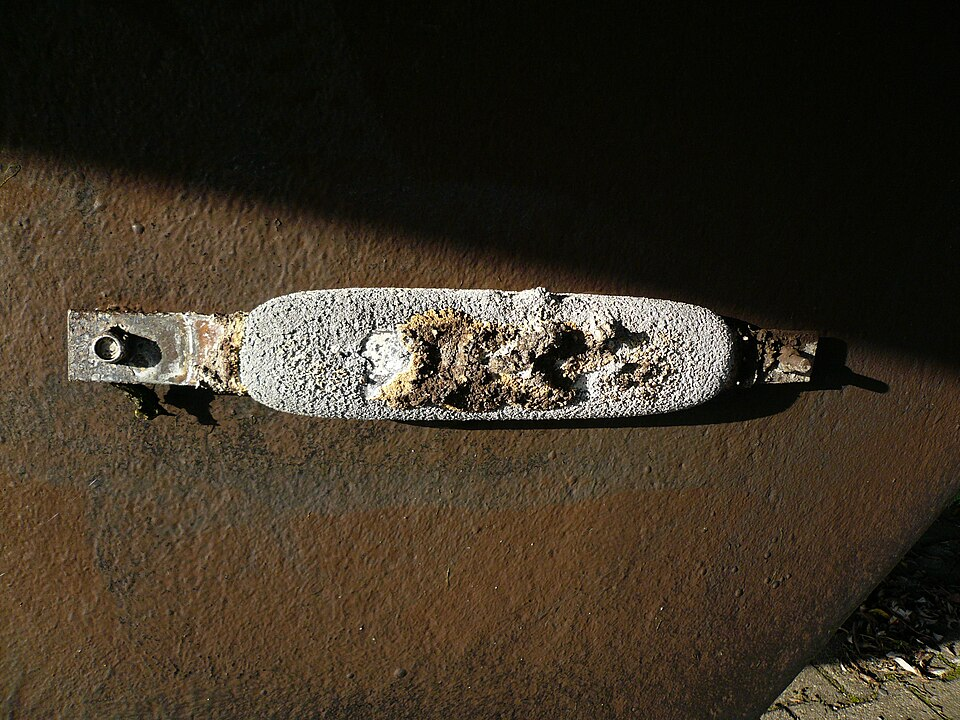
\includegraphics[width=0.5\linewidth]{images/book3/sacrificial-anode.jpg}

{\small Um \omterm{def:b2:corrosion:protection}{ânodo de sacrifício} de zinco aparafusado ao casco de aço de um
barco, após uma temporada na água: o zinco está corroído, e o aço em volta
dele, intacto. (Fotografia: Zwergelstern, CC BY-SA 3.0, Wikimedia Commons.)}
\end{omfigure}

\begin{omfigure}
\begin{tikzpicture}[font=\small, >={Stealth}, scale=1.35]
  \begin{scope}
    \fill[black!25] (0,0) rectangle (4,0.6);
    \fill[gray!55] (0,0.6) rectangle (1.7,0.8); \fill[gray!55] (2.3,0.6) rectangle (4,0.8);
    \fill[omDef!15] (0.8,0.8) .. controls (1.3,1.3) and (2.7,1.3) .. (3.2,0.8) -- (2.3,0.8) -- (2.3,0.6) -- (1.7,0.6) -- (1.7,0.8) -- cycle;
    \node[font=\scriptsize] at (2,-0.3) {aço galvanizado (camada de zinco)};
    \node[font=\scriptsize, align=center] at (2,1.6) {o zinco corrói,\\ o aço é protegido};
    \draw[->, omThm] (1.4,0.85) -- (1.8,0.65);
  \end{scope}
  \begin{scope}[xshift=5.5cm]
    \fill[black!25] (0,0) rectangle (4,0.6);
    \fill[gray!25] (0,0.6) rectangle (1.7,0.8); \fill[gray!25] (2.3,0.6) rectangle (4,0.8);
    \fill[omDef!15] (0.8,0.8) .. controls (1.3,1.3) and (2.7,1.3) .. (3.2,0.8) -- (2.3,0.8) -- (2.3,0.6) -- (1.7,0.6) -- (1.7,0.8) -- cycle;
    \fill[omProp] (1.75,0.6) rectangle (2.25,0.45);
    \node[font=\scriptsize] at (2,-0.3) {aço estanhado (camada de estanho)};
    \node[font=\scriptsize, align=center] at (2,1.6) {o aço corrói no risco,\\ depressa (ânodo pequeno)};
  \end{scope}
\end{tikzpicture}

{\small Um risco através de um revestimento metálico, esquemático. O zinco,
menos nobre que o ferro, torna-se o ânodo e protege o aço exposto, qualquer
que seja o tamanho do risco. O estanho, mais nobre que o ferro, torna-se um
grande cátodo em volta de um pequeno ânodo de aço, que corrói mais depressa
do que o aço nu.}
\end{omfigure}

\begin{method}[Escolher uma proteção]\label{met:b2:corrosion:choose-protection}
\begin{enumerate}
  \item Evite os pares galvânicos: isole os metais diferentes, ou faça do
        menos nobre o maior.
  \item Revista: um revestimento de barreira (pintura, estanho) só protege
        enquanto está intacto; um revestimento de sacrifício (zinco) protege
        mesmo quando riscado.
  \item Para uma estrutura no solo ou na água do mar, acrescente \omterm{def:b2:corrosion:protection}{proteção
        catódica}: \omterm{def:b2:corrosion:protection}{ânodos de sacrifício} para correntes pequenas ou água
        condutora, corrente impressa para estruturas longas ou solos
        resistivos.
  \item Não superproteja: um potencial baixo demais reduz a água a hidrogênio
        na estrutura, o que descola os revestimentos e pode fragilizar os
        aços de alta resistência.
\end{enumerate}
\end{method}

\section{Exercícios}

\begin{exercise}[$\star$]\label{exo:b2:corrosion:1}
O zinco corrói de modo uniforme sob uma densidade de corrente de \qty{2.0}{\micro A/cm^2}.
Calcule sua perda de espessura por ano ($\rho = \qty{7.13}{g/cm^3}$).
\end{exercise}

\begin{exercise}[$\star$]\label{exo:b2:corrosion:2}
Parafusos de aço fixam chapas de cobre em um telhado. Qual metal corrói? Mesma
pergunta para pregos de zinco em chapas de aço.
\end{exercise}

\begin{exercise}[$\star$]\label{exo:b2:corrosion:3}
Duas placas de aço são unidas por um parafuso e deixadas na água do mar. Onde
a corrosão se concentra, e por quê?
\end{exercise}

\begin{exercise}[$\star$]\label{exo:b2:corrosion:4}
Um balde galvanizado e uma lata estanhada são ambos riscados até o aço. Qual
deles enferruja no risco?
\end{exercise}

\begin{exercise}[$\star\star$]\label{exo:b2:corrosion:5}
No diagrama de Evans do ferro em água aerada, explique o que acontece com o
potencial e com a \omterm{def:b2:corrosion:uniform}{corrente de corrosão} quando a água é agitada e depois quando
ela é isenta de oxigênio.
\end{exercise}

\begin{exercise}[$\star\star$]\label{exo:b2:corrosion:6}
Um ânodo de zinco de \qty{5.0}{kg} protege o casco de um barco com uma corrente
de \qty{0.10}{A}, com um rendimento de 90~\% (dados do exercício). Quanto tempo
ele dura?
\end{exercise}

\begin{exercise}[$\star\star$]\label{exo:b2:corrosion:7}
Calcule a carga, em ampères-hora por quilograma, fornecida por ânodos de
zinco, magnésio e alumínio com 100~\% de rendimento, e os potenciais padrão de
seus pares a partir dos $\Delta_f G^\circ$ (\ce{Zn^2+} $-147.06$, \ce{Mg^2+} $-454.8$,
\ce{Al^3+} $-485$ \unit{kJ/mol}). Por que se prefere o magnésio em solos secos?
\end{exercise}

\begin{exercise}[$\star\star$]\label{exo:b2:corrosion:8}
Um duto enterrado precisa de \qty{2.0}{A} de corrente de proteção. O leito do
ânodo inerte tem uma resistência de \qty{4.0}{\ohm} em relação ao solo, e a
pilha exige mais \qty{1.5}{V} (dados do exercício). Calcule a tensão do
retificador e a energia elétrica por ano.
\end{exercise}

\begin{exercise}[$\star\star$]\label{exo:b2:corrosion:9}
Uma estaca de aço está fincada no mar. Explique por que ela corrói mais um
pouco abaixo da linha d'água, e não na própria linha d'água.
\end{exercise}

\begin{exercise}[$\star\star\star$]\label{exo:b2:corrosion:10}
Explique, com a curva passiva, por que o aço inoxidável resiste à água aerada,
mas pode sofrer pites na água do mar, e por que um pite, uma vez iniciado,
cresce mais em profundidade do que em largura.
\end{exercise}

\begin{exercise}[$\star\star\star$]\label{exo:b2:corrosion:11}
Uma conexão de cobre é rosqueada em um tubo de aço que transporta água aerada.
A densidade de \omterm{def:b2:current-potential-curves:limiting-current}{corrente limite} do oxigênio é de \qty{5}{\micro A/cm^2} em toda
superfície molhada; o cobre oferece \qty{20}{cm^2} e o aço perto da junta
\qty{2}{cm^2} (dados do exercício). Estime a \omterm{def:b2:corrosion:uniform}{corrente de corrosão} do aço e sua
perda de espessura por ano perto da junta.
\end{exercise}

\begin{exercise}[$\star\star\star$]\label{exo:b2:corrosion:12}
Usando o diagrama E--pH do ferro e as curvas da água, explique por que o
potencial de uma estrutura de aço protegida deve ser mantido abaixo de cerca de
\qty{-0.6}{V}, mas não muito abaixo de \qty{-1}{V}, em água neutra.
\end{exercise}

\section{Problema: Proteger um duto}

\begin{problem}[{Problema de fim de semana --- a corrosão de um tubo de aço nu em
solo úmido, a escolha de um metal de sacrifício, o magnésio necessário para
vinte anos e a alternativa da corrente impressa}]
\label{pb:b2:corrosion:1}
Um duto de aço de \qty{10.0}{km} de comprimento e \qty{0.30}{m} de diâmetro está
enterrado em solo úmido. Dados: ferro $M = \qty{55.845}{g/mol}$, $\rho = \qty{7.87}{g/cm^3}$;
magnésio $M = \qty{24.305}{g/mol}$; $\Delta_f G^\circ$ (\unit{kJ/mol}): \ce{Fe^2+}
$-78.90$, \ce{Zn^2+} $-147.06$, \ce{Mg^2+} $-454.8$, \ce{Al^3+} $-485$. Dados do
exercício: densidade de \omterm{def:b2:corrosion:uniform}{corrente de corrosão} do aço nu nesse solo \qty{10}{\micro
A/cm^2}; densidade de corrente de projeto para a proteção do aço nu
\qty{20}{mA/m^2}; o revestimento deixa 1.0~\% da superfície nua; ânodos de
magnésio de \qty{15}{kg}, rendimento 50~\%; resistência do leito anódico da
corrente impressa \qty{5.0}{\ohm}.
% ledger: aw:Fe, rho:Fe, aw:Mg, dfg:Fe2+_ao, dfg:Zn2+_ao, dfg:Mg2+_ao, dfg:Al3+_ao, const:F

\medskip
\noindent\textbf{Parte I --- O tubo nu.}
\begin{enumerate}
  \item Escreva as reações anódica e catódica no tubo.
  \item Por que a \omterm{def:b2:corrosion:uniform}{corrente de corrosão} é fixada pelo suprimento de oxigênio?
  \item Calcule a massa de ferro perdida por metro quadrado e por ano.
  \item Calcule a perda de espessura da parede por ano.
  \item Quanto tempo o tubo nu levaria para perder metade de uma parede de \qty{8}{mm}?
  \item Por que o tubo real falha mais cedo, em alguns pontos?
\end{enumerate}

\medskip
\noindent\textbf{Parte II --- O metal do ânodo.}
\begin{enumerate}[resume]
  \item Calcule os potenciais padrão dos pares do ferro, do zinco, do magnésio
        e do alumínio.
  \item Quais metais podem proteger o ferro como \omterm{def:b2:corrosion:protection}{ânodos de sacrifício}?
  \item Por que o alumínio é pouco usado em solos?
  \item Por que se prefere o magnésio ao zinco em um solo de alta resistividade?
  \item Calcule a massa de magnésio consumida por ampère e por ano.
\end{enumerate}

\medskip
\noindent\textbf{Parte III --- O projeto.}
\begin{enumerate}[resume]
  \item Calcule a superfície externa do tubo.
  \item Calcule a superfície nua deixada pelo revestimento.
  \item Calcule a corrente de proteção.
  \item Calcule a carga necessária para vinte anos.
  \item Calcule a massa de magnésio necessária.
  \item Quantos ânodos são necessários?
  \item Por que eles são distribuídos ao longo do tubo, em vez de enterrados
        em um único ponto?
\end{enumerate}

\medskip
\noindent\textbf{Parte IV --- A corrente impressa.}
\begin{enumerate}[resume]
  \item Descreva a alternativa da corrente impressa.
  \item Estime a tensão do retificador a partir da resistência do leito
        anódico, acrescentando \qty{1.5}{V} para os eletrodos.
  \item Calcule a energia elétrica consumida por ano.
  \item O que dá errado se o tubo for superprotegido?
  \item Abaixo de que potencial o ferro é imune em água neutra, tomando uma
        concentração de ferro(II) de \qty{1e-6}{mol/L}?
  \item Dê a massa de ânodos de magnésio necessária para vinte anos.
\end{enumerate}
\end{problem}
